\section{Opgave 3}
\subsection{Beskrivelse og Design}
Der ønskes en implementation af det klassiske spil vektorrally,
hvor man kan styre en vektor rundt på en bane ved hjælp af numpad tasterne.
Udover dette har vi også valgt at implementere følgene i programmet:
\begin{itemize}
  \item Kode der registrerer når vektoren kører den forkerte vej
  \item Kode der registrerer når vektoren passerer målstregen og angiver antal træk
  \item Kode der muliggør at man kan spille mod computeren
  \item Et separat editeringsprogram hvor en bane kan kreeres og gemmes til brug i hovedeprogrammet.
\end{itemize}

Vi har valgt at ændre styre-mekanismen, så man ikke behøver at trykke \emph{enter} efter at vælge retning med numpad.
Vi blev simpelt hen trætte af det ekstra taste tryk.

Der er således skrevet 2 programmer. Det ville være muligt at sætte dem sammen med et menu-system,
men dette har vi udeladt, da programmets funktionalitet ikke ville være synderligt ændret i forhold til den ekstra implementeringstid.
De 2 programmer deler et tegnesystem hvor der kreeres et 640x480 vindue,
men selvom vinduet har en fikseret størrelse er der mulighed for at have skalerede baner da banerne har eget koordinatsystem.
Man kan derfor spille på store eller små baner i et vindue der ikke ændrer størrelse.

De elementer der tegnes er alle af klassen \emph{GameObject}. %klasse eller type?
Dette er en klasse der indeholder alle de spilelementer der skal tegnes og som kan interagere med hinanden i spillet.
Børn af GameObject er f.eks. Player, GhostPlayer, Checkpoint og Wall. Hvert objekt i spillet har et ID
(et nøgleord, der fortæller, hvad type objektet er), en update metode og en render metode.
Dette sørger GameObject for er opfyldt. GameObject behøver dog ikke at være et interface,
og dermed tvinge de andre klasser til at implementere disse metoder,
men indeholder i stedet tomme placeholder metoder der medfører.
Dette medfører at lister af GameObjects kan laves,
en liste kan hurtigt gennemløbes og dermed gøres det nemt, at opdaterer alle objekter.

I programmet foregår alt efter initaliseringen  i et main loop hvor update() og render() metoderne kaldes gang på gang.

\subsubsection{Spilprogrammet}
RaceTrack programmet er hovedeprogrammet hvor det er muligt at spille vektorrally. Programflowet er:
\begin{enumerate}
  \item Spørg spilleren hvilken bane han/hun gerne vil køre på
  \item Initaliser spillervinduet med den valgte bane
  \item Lad spilleren bevæge sig rundt indtil han/hun støder ind i en væg eller passerer målstregen
  \item Spørg spilleren om spillet ønskes fortset, hvis ja så gå til 1, hvis nej så stop.
\end{enumerate}
Rundt på banen er der placeret checkpoints der fungerer som sub-målstreger og sikrer at spilleren kører den rigtige vej igennem en bane.
Denne åbner muligheden for baner der ikke er cirkulære i deres udformning.
Spilleren får en advarsel hvis han kører væk fra næste checkpoint i  mere end 2 træk.
Støder spilleren ind i en mur, eller færdiggør spilleren banen, spørger programmet spilleren om han/hun ønsker at fortsætte.
Er svaret ja, genstartets spillet i samme bane.

\subsubsection{Computerspiller}
En stor del af ``ekstra'' funktionerne er belvet implimenteret for at muliggøre en computer modspiller.
Computerspilleren er implimenteret som en darwinistisk pathfinding.
Der oprettes en \emph{agent manager}, denne laver agenter, der kører tilfældigt rundt,
indtil de støder ind i en mur, eller kører gennem en checkpoint.
Kører de ind i en checkpoint, undersøgets det, om dette stemmer overens med den checkpoint de, ifølge ``manageren'' skal ``lede efter''.

Når nok agentser har fundet den checkpoint der ``ledes efter'', vælges de hurtigste af dem til at danne basis for en ny generation af agenter.

Der er også mulighed for at lade agenterne kører et antal checkpoints længere,
for fx. imødegå skarpe sving; men dette giver en langsommere aloritme.

\begin{lstlisting}
(1)
	Et "GameObject", "AgentMananger" tilføjes listen af GameObjects
	Antallet af checkpoints, hver agent skal passerer udregnes
	AgentManager laver en liste af "AgentPlayer"s, 5000-20.000.
(2)
	For hver AgentPlayer gøres nu følgende:
		Den prædefinererde sti muteres.
		
		Agenten "kører" af stien indtil:
			den kører ind i en mur,
			den kører den forkerte vej,
			eller den passerer den sidste checkpoint, den skal
		
		"Dør" en agent, laves en ny.
		
		Ved en checkpoint gemmes listen af skridt, der førte derhen
		  og tiden dettte tog i en liste hos "AgentManager"
(3)
	Når nok agenter har passeret checkpointen,
	  vælges et antal af de hurtigste stier og disse bruges
	  som den prædefinerede sti for en ny generation
	Antallet af checkpoints der skal passeret opdateres
	Der laves en ny liste af agenter og startes forfra ved (2)
	  indtil banen er kørt igennem.

	Når en sti er fundet, der gør hele banen rundt,
	  køres et antal optimeringsrunder.
(4)
	En "GhostPlayer", en spiller, der rykker samtiding med brugeren,
	  efter et prædefineret mønster, oprettes, med den hurtigste af stierne.
\end{lstlisting}

Programmet pauses \emph{ikke} mens computerspilleren finder sin sti, så ønsker man at spille mod denne,
skal man vente til den ``onde'' sorte spiller, med rødt spor bliver lavet. 


\subsubsection{Baneeditor programmet}
Køres MapCreator programmet åbnes et vindue hvor det er muligt at tegne sin egen bane og gemme den til senere gennemkørsler i RaceTrack programmet.
Der kan interageres med programmet med følgene keybindings:
\begin{itemize}
  \item SHIFT-W Starter en væg ved det gridpunkt der ligger nærmest ved cursoren, væggen ender der hvor brugeren klikker med musen.
  \item SHIFT+C Samme som for en væg, skaber bare et checkpoint i stedet. Når banen gennemkøres skal checkpoints passeres i den rækkefølge de blev placeret i MapCreator.
  \item SHIFT+S Placerer spillerens startposition under cursoren.
  \item ESCAPE Gemmer banen i maps folderen med filnavnet mapN.map hvor N er det laveste tal der ikke findes i folderen i forvejen.
\end{itemize}
Er der ikke placeret både et checkpoint og en wall vil programmet ikke gemme banen. Det er dog op til brugeren selv om han/hun vil placere et startpoint, dette defaulter til (0,0) og kan senere ændres i .map filen.

\subsection{Programtest}

\subsubsection{Test af RaceTrack}
Følgende ting testes i \emph{RaceTrack}:
\begin{itemize}
  \item Kode der registrerer når vektoren kører den forkerte vej
  \item Kode der registrerer når vektoren passerer målstregen og angiver antal træk
  \item Kode der registrerer når vektoren kører ind i en mur
\end{itemize}

\paragraph{Vektoren kører den forkerte vej}
I det øjeblik hvor spilleren drejer til venstre, væk fra næste checkpoint, printes:
\begin{lstlisting}
WRONG WAY!
\end{lstlisting}
til konsollen, se figur~\ref{fig:wrongway}
\begin{figure}[h!]
	\centering
	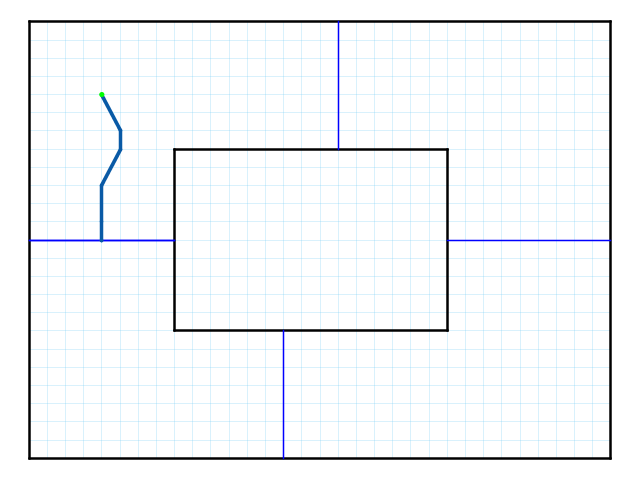
\includegraphics[width=0.5\textwidth]{wrongway}
		\caption{I det øjeblik hvor spilleren drejer til venstre, væk fra næste checkpoint, printes ``WRONG WAY!'' til konsollen}\label{fig:wrongway}
\end{figure}

\paragraph{Vektoren kører i mål} Figur~\ref{fig:maal}
I det øjeblik hvor spilleren har passeret alle checkpoints (den sidste er oveni den første, der hvor man starter) printes følgende til konsollen:
\begin{lstlisting}
You sir, or ma'am, win "one million" internetz!
Well not really; men du klarede det på:
23 træk.
Game has ended. Type "more!" to play again.
type anything else to be a wuz and quit.
\end{lstlisting}
Antallet af skridt er selvfølgelig afhængit af, hvor godt man klarer sig.
\begin{figure}[h!]
	\centering
	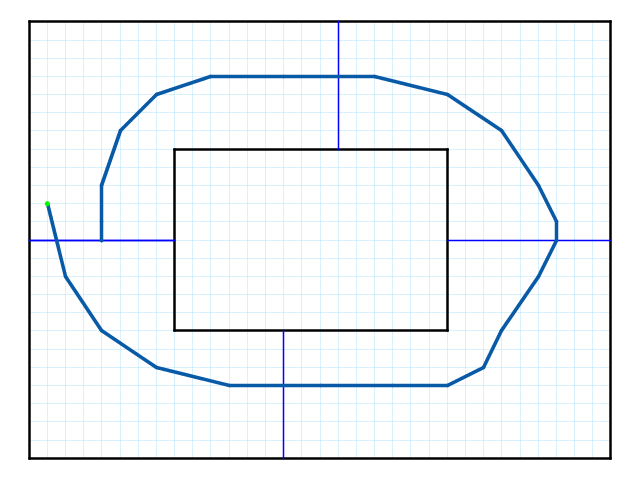
\includegraphics[width=0.5\textwidth]{maal}
		\caption{Spilleren kører i mål}\label{fig:maal}
\end{figure}

\paragraph{Vektoren kører i en væg} Figur~\ref{fig:vaeg}
I det øjeblik hvor spilleren rammer en væg printes følgende til konsollen:
\begin{lstlisting}
Derp °_o
Du døde vist
Ej hvor flot du smadrede din "vektor" på bare:
15 træk.
Game has ended. Type "more!" to play again.
type anything else to be a wuz and quit.
\end{lstlisting}
Antallet af skridt er selvfølgelig afhængit af, hvor dårligt man klarer sig.
\begin{figure}[h!]
	\centering
	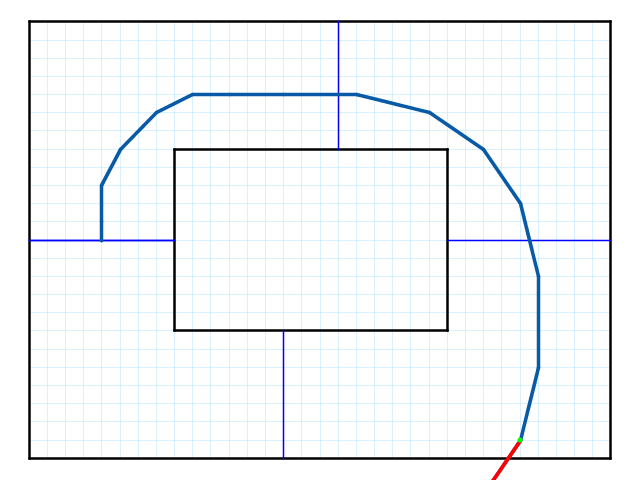
\includegraphics[width=0.5\textwidth]{vaeg}
		\caption{Spilleren kører i mål}\label{fig:vaeg}
\end{figure}

\subsubsection{test af AgentManager}
Det er muligt undervejs at tegne de agenter, der er i live, men da dette tager lang tid
(et par tusinde agenter, er mange linjer, der skal tegnes) er dette en debug feature, 
der kan slåes til ved at trykke \emph{d}.

For en simplel bane (banen \emph{simple}) ser et billede af agenterne undervejs ud som i figur~\ref{fig:simpleD},
den færdige rute er at se i figur~\ref{fig:simpleF} (spilleren står stille ved at trykke på \emph{5})

\begin{figure}[h!]
	\centering
	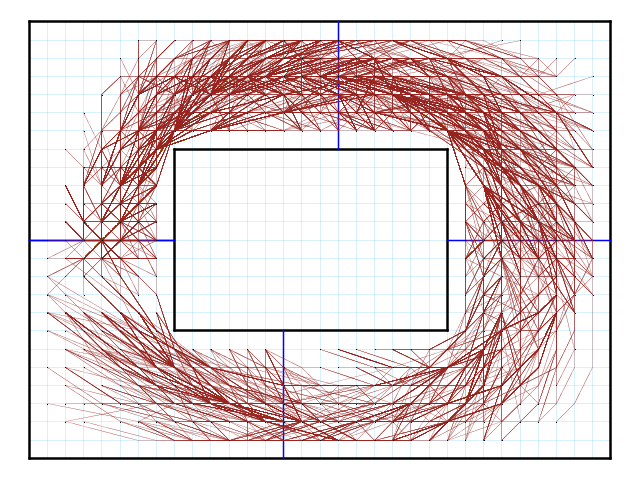
\includegraphics[width=0.5\textwidth]{simpleD}
		\caption{Debug billede fra banen \emph{simple}}\label{fig:simpleD}
\end{figure}

\begin{figure}[h!]
	\centering
	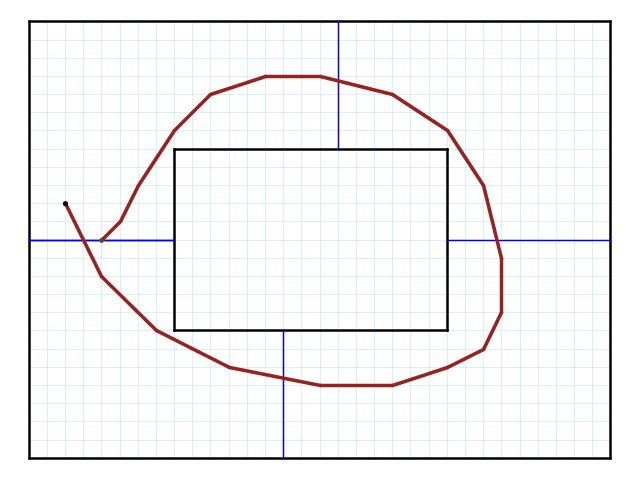
\includegraphics[width=0.5\textwidth]{simpleF}
		\caption{Færdig rute fra banen \emph{simple}, længden er 19 skridt.}\label{fig:simpleF}
\end{figure}

For en mere kompliceret bane (banen \emph{complicated}) ser et billede af agenterne undervejs ud som i figur~\ref{fig:compD},
den færdige rute er at se i figur~\ref{fig:compF} (spilleren står stille ved at trykke på \emph{5})

\begin{figure}[h!]
	\centering
	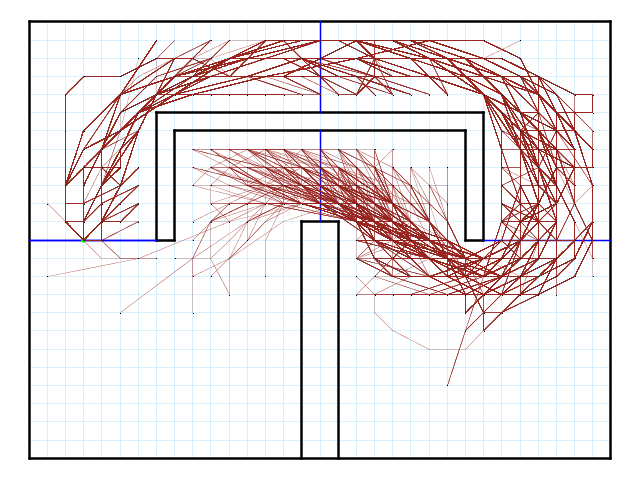
\includegraphics[width=0.5\textwidth]{compD}
		\caption{Debug billede fra banen \emph{complicated}}\label{fig:compD}
\end{figure}

\begin{figure}[h!]
	\centering
	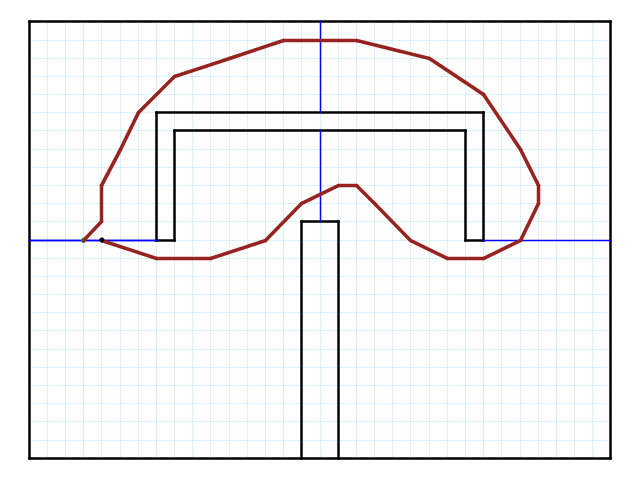
\includegraphics[width=0.5\textwidth]{compF}
		\caption{Færdig rute fra banen \emph{complicated}, længden er 25 skridt.}\label{fig:compF}
\end{figure}

\clearpage

\subsubsection{Test af baneeditor}
Følgende ting er testet i MapCreator
\begin{itemize}
\item Programmet godtager ikke negative grid-størrelser.
\item Programmet gemmer ikke baner uden checkpoints og mure.
\end{itemize}

Det er ikke testet hvad der sker hvis der bliver smidt en exception imens programmet er igang til at skrive til en fil. Programmet vil dog afbryde saveToFile() metoden hvis dette sker og den korrupte mapfil skal herefter slettes manuelt.\\
\\
Når mappet skal loades til gennemkørsel er det testet at:
\begin{itemize}
\item Programmet tjekker at filen eksisterer og loader ikke filer der ikke eksisterer.
\item Programmet gør intet med linjer der ikke har et accepteret element token.
\end{itemize}
Stoppes programudførslen pga. en exception imens banen loades fra en fil vil de allerede loadede objekter blive slettet fra objektlisten og brugeren blive bedt om at prøve at indtaste et nyt map navn.\\
Det er ikke muligt at garantere for at programudførslen vil foregå på denne måde,men da disse tests er successfulde skal ekstra bugs findes ved videre playtesting.
\\
Til slut skal det nævnes at det selvfølgelig er muligt at editere map filerne i hånden og derved skabe sjove situationer. Men dette er der ikke lavet safeguards imod da det ikke vurderes som vigtigt i denne applikation.
